% XCircuit output "DSM_circuit_model.tex" for LaTeX input from DSM_circuit_model.ps
\def\putbox#1#2#3{\makebox[0in][l]{\makebox[#1][l]{}\raisebox{\baselineskip}[0in][0in]{\raisebox{#2}[0in][0in]{#3}}}}
\def\rightbox#1{\makebox[0in][r]{#1}}
\def\centbox#1{\makebox[0in]{#1}}
\def\topbox#1{\raisebox{-\baselineskip}[0in][0in]{#1}}
\def\midbox#1{\raisebox{-0.5\baselineskip}[0in][0in]{#1}}
\begin{flushleft}
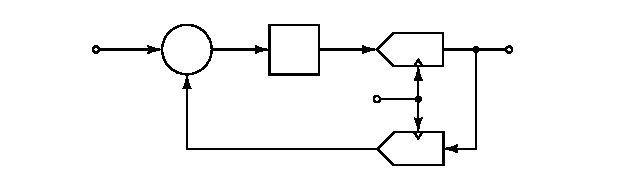
\epsfig{file=DSM_circuit_model.ps}\\
% translate x=1132 y=514 scale 0.25
\putbox{1.14in}{0.83in}{\centbox{\midbox{\begin{LARGE}$\Sigma$\end{LARGE}}}}%
\putbox{3.48in}{0.88in}{\centbox{\midbox{\begin{small}$y(n)$\end{small}}}}%
\putbox{2.66in}{0.20in}{\centbox{\midbox{DAC}}}%
\putbox{2.66in}{0.86in}{\centbox{\midbox{ADC}}}%
\putbox{1.08in}{0.66in}{\centbox{\midbox{-}}}%
\putbox{1.85in}{0.87in}{\centbox{\midbox{\begin{large}$\int$\end{large}}}}%
\putbox{2.29in}{0.55in}{\centbox{\midbox{\begin{small}$f_s$\end{small}}}}%
\putbox{0.42in}{0.88in}{\centbox{\midbox{\begin{small}$x(t)$\end{small}}}}%
\end{flushleft}
